\documentclass{article}

\usepackage{graphicx}
\usepackage{float}
\usepackage[font=small,labelfont=bf]{caption}
\usepackage{geometry}
\usepackage{fancyhdr}
\usepackage{appendix}
\usepackage{amsmath}
\usepackage{amsthm}
\usepackage{amsfonts}
\usepackage{amssymb}
\usepackage{stmaryrd}
\usepackage{mathrsfs}
\usepackage{array}
\usepackage{multirow}
\usepackage{makecell}
\usepackage{listings}
\usepackage{xcolor}
\usepackage{tabto}
% \usepackage{hyperref}
\usepackage{titlesec}
\usepackage[hidelinks]{hyperref}
\usepackage[french]{babel}
\usepackage[utf8]{inputenc}
\usepackage[T1]{fontenc}
\usepackage{xspace}
\usepackage{pxfonts}


\pagestyle{fancy}
\lhead{Burgalat Eliot - Garcia Tom}
\rhead{MPI - 2024}


\definecolor{codegreen}{rgb}{0,0.6,0}
\definecolor{codeblue}{rgb}{0,0,0.6}
\definecolor{codegray}{rgb}{0.5,0.5,0.5}
\definecolor{codepurple}{rgb}{0.58,0,0.82}
\definecolor{backcolour}{rgb}{0.95,0.95,0.92}


\lstdefinestyle{mystyle}{
    % backgroundcolor=\color{backcolour},  
    commentstyle=\color{codegreen},
    keywordstyle=\color{blue},
    numberstyle=\tiny\color{codegray},
    numbers=left,                   
    stringstyle=\color{codegreen},
    basicstyle=\ttfamily\small,
    showstringspaces=false,
    % breakatwhitespace=false,
    % breaklines=true,                
    % captionpos=b,                   
    % keepspaces=true,                
    % numbersep=5pt,                 
    % showspaces=false,               
    % showtabs=false,                 
    % tabsize=2
}
\lstset{style=mystyle}




\setcellgapes{1pt}
\makegapedcells
\newcolumntype{R}[1]{>{\raggedleft\arraybackslash}b{#1}}
\newcolumntype{L}[1]{>{\raggedright\arraybackslash}b{#1}}
\newcolumntype{C}[1]{>{\centering\arraybackslash}b{#1}}

\title{\underline{Ray Marching}}
\date{}
\author{Burgalat - Garcia}
\renewcommand*\contentsname{Sommaire}


\geometry{paperwidth=24cm}

% --- Debut du doc --- %
\begin{document}

\maketitle
\tableofcontents
\clearpage

\section{Tout commence par le commencement}
\subsection{Le principe du Ray Marching}

Le Ray marching consiste a faire du rendu 3D grace a des Signed Distances Functions (SDF). 
Qui sont des fonctions qui calculent la distance entre un point et un objet, avec une distance négative des que le point se trouve a l'interieur de l'objet.

Pour cela, pour chaque pixel de la camera on va envoyer un rayon depuis la camera passant par ce pixel. 
Pour savoir quel est la distance maximal que ce rayon peut parcourir, on calcule la distance minimal a tous les objets de la scene. 
On peut donc avancer de cette distance et on repette cela jusqu'a atteindre un objet ou dépasser une distance minimal. 
On peut donc colorier le pixel en fonction du resultat.

\begin{figure}[H]
    \begin{center}
        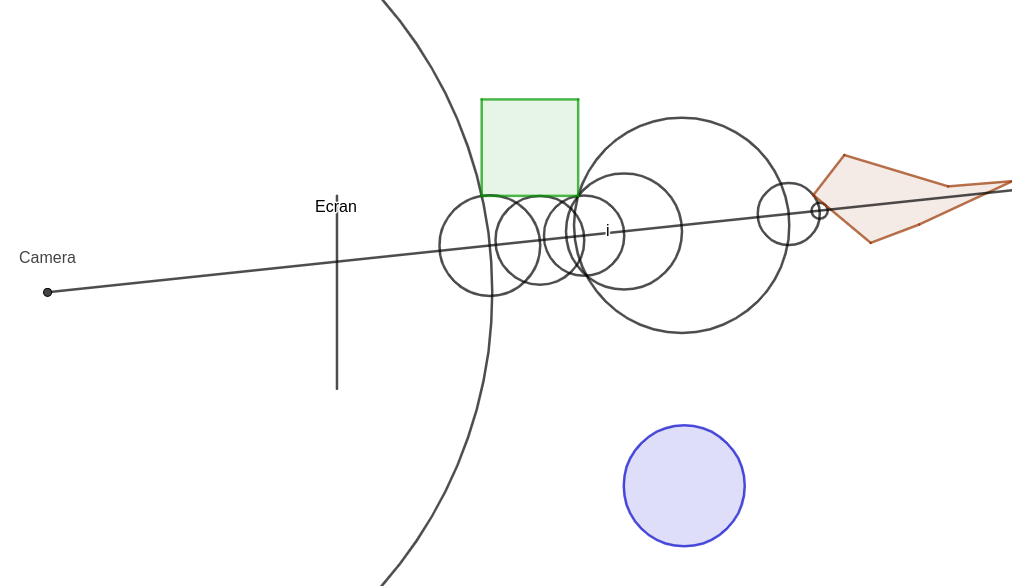
\includegraphics[width=10cm]{images/Shema_1_ray_marching_2d.png}\caption{Schéma rayon Ray Marching en 2D}
    \end{center}
\end{figure}



\subsection{Affichage}

\subsection{SdF}
Le principe de la Signed Distance Function (SdF) est de calculer la distance entre un point et un objet, avec une distance négative des que le point se trouve a l'interieur de l'objet.
\smallskip

On peut donc donner à chaque forme de base une fonction distance afin de permettre, lors du lancer de chaque rayon, 
de savoir si le rayon atteint l'objet (la SdF renverra une valeur négative lorsqu'il arrivera à un point dans l'objet),
où s'il ne touche pas (à partir d'une certaine distance atteinte par le rayon, on considère qu'aucun objet est atteint et alors on renvoie un fond uniforme).
\medskip 

\underline{Exemple de la sphère :}
\begin{lstlisting}
float SDF_sphere(coord p, coord centre, float rayon){
  float dist = 
    sqrt((p.x-centre.x)*(p.x-centre.x)+(p.y-centre.y)*(p.y-centre.y)+(p.z-centre.z)*(p.z-centre.z));
  return dist - rayon;
}
\end{lstlisting}
\medskip 

Les formes de base implémentées sont : 
\begin{itemize}
    \item Plan
    \item Sphère
    \item Tor
    \item Boite
    \item Pyramide 
    \item Cylindre
\end{itemize}

\bigskip
\underline{Exemple du triangle :}
\medskip

Le triangle est l'une des forme les plus importante en modélisation 3D car tous objet peut etre réprensenté facilement (avec plus ou moins de précision) grace a seulement des triangles.

\subsection{Affichage des lumières et ombres}

\section{Opérations}
\subsection{Opérations de base :}
\subsubsection{Union}
Afin de procéder l'union entre 2 objets/formes, il suffit de considérer à chaque fois la plus faible 
valeur entre la sdf d'un objet et celle de l'autre, ce qui nous permettra, pour chaque rayon de lancé,
de capter la présence de la première forme présente sur son chemin.

\begin{lstlisting}
float UnionSDF (float d1, float d2){
    return MIN(d1,d2);
}
\end{lstlisting}

\subsubsection{Intersection}
Au contraire pour l'Intersection, il suffit de considérer la distance maximale :
Si un des 2 objets n'est pas présent, la fonction intersection renverra toujours le maximum des 2 sdf,
soit une distance positive et ainsi aucun objet ne sera atteint. Pour les points sur lesquels les 2 objets sont présents,
la fonction renverra bien une distance négative (car les 2 le sont) à l'arrivée du rayon en ce point.

\begin{lstlisting}
float IntersectSDF (float d1, float d2){
    return MAX(d1,d2);
}
\end{lstlisting}

\subsubsection{Soustarction}
La soustraction de F1 par F2 se traduit à $F1_{\backslash F2}$

Il suffit donc de considérer les points où la sdf de F1 est positive, et celle de F2 négative.

\begin{lstlisting}
float SubstractSDF (float d1, float d2){
    return MAX(d1, -d2); 
}
\end{lstlisting}

\subsubsection{Rotations}

\subsection{Amélioration des effets}
\subsubsection{Fonctions de lissage - Smooth}

\section{Optimisations}

\subsection{Bounding Volumes Hierarchy (BVH-Trees)}
Arbres K-dimensionnels de priorisation des SdF

\subsection{Multi-threading}


\subsection{Chiffres}

\subsection{Méthode naive}
Nous avons sélectionner plusieurs scenes de references pour visualiser les performances de notre programme.

[insert scene]

Premiere implementation (sans reel opti) : 

[mettre des graphiques en camenbert et tout ca]

\section{Liens PDF utilisés}

\underline{\href{https://ieeexplore-ieee-org.gorgone.univ-toulouse.fr/document/5457293}{Documentation / Explication de OpenCL}}
\smallskip 

\underline{\href{https://iquilezles.org/}{Site de iq (el crackito du Ray Marching)}}

\end{document}